\chapter{三维空间中的薛定谔方程}\label{ch:b3:schrodinger-three-dimensions}

现代电视机的屏幕由极小的晶体发光，这些晶体小到
其\emph{尺寸}决定其颜色：一颗硒化镉颗粒直径
4 纳米时发红光，同一物质在 2 纳米时
则发蓝绿光。化学成分毫无差别——区别只在于
约束电子的“盒子”大小。本科二年级分册以
一维量子力学收尾：直线上的波函数、势阱、
势垒与隧道效应。但电子生活在三维空间中，而
从直线到空间的跨越带来了真正全新的物理：
概率以流的形式在空间中输运，盒子的能级
会因\emph{简并}而堆积，揭示其对称性；状态必须
被\emph{计数}——这一计数日后将支撑整个统计
物理——而球对称问题在最简单的情形下可化为
关于半径的、伪装成一维的方程。本章将完成
这些步骤，其核心内容是电视机中的量子点与
自然界中最轻的原子核。

\section{空间中的波函数}

\begin{definition}[三维空间中的波函数与概率]\label{def:b3:schrodinger-three-dimensions:psi3d}
\index{波函数!三维}
粒子的状态是一个复值场 $\psi(\vect r, t)$，满足
玻恩定则
\[
\dd\mathcal P = |\psi(\vect r, t)|^2\,\dd^3r , \qquad
\int|\psi|^2\,\dd^3r = 1 ,
\]
其演化由薛定谔方程描述，其中用拉普拉斯算子
代替二阶导数：
\[
\iu\hbar\,\frac{\partial\psi}{\partial t}
 = -\frac{\hbar^2}{2m}\,\Delta\psi + V(\vect r)\,\psi ,
\qquad
\Delta = \frac{\partial^2}{\partial x^2} +
\frac{\partial^2}{\partial y^2} + \frac{\partial^2}{\partial z^2} .
\]
本科二年级分册所建立的全部结论原样保留：
线性与叠加原理，定态
$\varphi(\vect r)\,\eu^{-\iu Et/\hbar}$，满足
$-\tfrac{\hbar^2}{2m}\Delta\varphi + V\varphi = E\varphi$，以及
动量算符，此时为梯度 $\hat{\vect p} =
-\iu\hbar\vect\nabla$。
\end{definition}

\begin{proposition}[概率流：流密度]\label{prop:b3:schrodinger-three-dimensions:current}
\index{概率流}
密度 $\rho = |\psi|^2$ 满足连续性方程，
\[
\frac{\partial\rho}{\partial t} + \operatorname{div}\vect\jmath = 0 ,
\qquad
\vect\jmath = \frac{\hbar}{m}\,
\operatorname{Im}\big(\psi^*\vect\nabla\psi\big) :
\]
概率局域守恒，由流
$\vect\jmath$——对平面波 $A\eu^{\iu\vect k\cdot\vect r}$，
$\vect\jmath = |A|^2\hbar\vect k/m = \rho\vect v$，为匀速流动；
对任意实值 $\varphi$，$\vect\jmath = \vect 0$：束缚
定态不携带净流。
\end{proposition}

\begin{proof}
与一维情形相同：由方程及其共轭求 $\partial_t(\psi^*\psi)$；
势能项相消，而 $(\iu\hbar/2m)
(\psi^*\Delta\psi - \psi\Delta\psi^*) =
-\operatorname{div}\big[(\hbar/m)\operatorname{Im}(\psi^*\vect\nabla
\psi)\big]$ 由散度的乘积法则得出。
\end{proof}

\begin{omfigure}
\begin{tikzpicture}[font=\small, >=Stealth]
  % plane wave current
  \begin{scope}
    \foreach \y in {0.3,0.9,1.5,2.1}
      \foreach \x in {0.2,1.2,2.2,3.2}
        \draw[->, omDef] (\x,\y) -- (\x+0.62,\y);
    \foreach \x in {0.55,1.55,2.55,3.55}
      \draw[omExo!60, dashed] (\x,-0.05) -- (\x,2.45);
    \node at (1.95,-0.62) {平面波：匀速流 $\rho\vect v$};
  \end{scope}
  % vortex-free bound state
  \begin{scope}[xshift=7.6cm]
    \draw[omThm, thick] (1.7,1.2) circle (1.35);
    \draw[omThm!50, thick] (1.7,1.2) circle (0.75);
    \node[omThm] at (1.7,1.2) {$\varphi$ 实};
    \node at (1.85,-0.62) {束缚态：处处 $\vect\jmath = \vect 0$};
  \end{scope}
\end{tikzpicture}

{\small 概率流：行波像流体一样输运其
密度；实值（束缚、定态）波函数
则静止不动——原子中的电子云并不
环流，除非状态为复值。}
\end{omfigure}

\section{盒子、简并与状态计数}

\begin{theorem}[分离变量法]\label{thm:b3:schrodinger-three-dimensions:separation}
\index{分离变量法}
若势能可分解为 $V = V_1(x) + V_2(y) + V_3(z)$，则
定态可取为乘积形式
$\varphi(\vect r) = \varphi_1(x)\,\varphi_2(y)\,\varphi_3(z)$，其中
每个因子满足各自的一维问题，且能量
\emph{相加}：$E = E_1 + E_2 + E_3$。在这类情形中，三维问题
即三次一维问题。
\end{theorem}

\begin{proof}
将乘积代入定态方程，并除以
$\varphi$：三个单变量表达式之和等于
常数 $E$，故每一项分别为常数。每个状态都是
此类乘积的叠加，这源于一维
解的完备性，在本阶段不加证明地承认。
\end{proof}

\begin{proposition}[立方箱及其简并]\label{prop:b3:schrodinger-three-dimensions:box}
\index{简并}
边长为 $a$、壁不可穿透的箱中，态由
三个正整数标记，
\[
\varphi_{n_1n_2n_3} \propto
\sin\frac{n_1\pi x}{a}\sin\frac{n_2\pi y}{a}\sin\frac{n_3\pi z}{a} ,
\qquad
E = \frac{h^2}{8ma^2}\,(n_1^2 + n_2^2 + n_3^2) .
\]
不同的态现在共享能量：能级 $(2,1,1)$ 有
三重重复，$(1,2,1)$ 与 $(1,1,2)$ 是具有相同 $E$ 的
物理上不同的态。这种\emph{简并}是
对称性的标志——此处即箱子三条轴之间可互换；
将箱子稍微压扁，三重态便会分裂。
\end{proposition}

\begin{proof}
对三个无限深势阱分离变量（见本科二年级分册）；
能量相加。
\end{proof}

\begin{omfigure}
\begin{tikzpicture}[font=\small]
  \draw[->] (0,0) -- (0,6.1);
  \node[anchor=south] at (0,6.1) {$E\,/\,\dfrac{h^2}{8ma^2}$};
  \foreach \e/\lab/\deg in {3/{(1,1,1)}/1, 6/{(2,1,1)}/3, 9/{(2,2,1)}/3,
      11/{(3,1,1)}/3, 12/{(2,2,2)}/1, 14/{(3,2,1)}/6}
    {\draw[very thick, omDef] (0.6,\e*0.42) -- (2.6,\e*0.42);
     \node[anchor=west] at (2.75,\e*0.42) {$\e$\quad\lab, 简并度 \deg};}
\end{tikzpicture}

{\small 立方箱的最低能级：能量以 $h^2/8ma^2$ 为单位，
并标出各自的量子数。$n_i$ 不相等时的置换给出
简并三重态与六重态——这是
立方对称性的特征。}
\end{omfigure}

\begin{proposition}[态的计数]\label{prop:b3:schrodinger-three-dimensions:counting}
\index{态密度}
能量低于 $E$ 的箱中态数，当 $E$ 较大时，
\[
N(E) \approx \frac{V}{6\pi^2}\Big(\frac{2mE}{\hbar^2}\Big)^{3/2} ,
\qquad V = a^3 :
\]
与体积成正比，并与 $E^{3/2}$ 成正比。等价地，
相空间中每个体积 $h^3$ 容纳一个量子态——
即玻尔–索末菲胞，见
\cref{ch:b3:hamiltonian-mechanics}，此处予以推导。这一计数
是本册后续统计物理与固体物理的基础：
金属中的电子、腔内的光子、热物体的辉光
都由此出发。
\end{proposition}

\begin{proof}
态即正卦限中的格点 $(n_1, n_2, n_3)$；
条件 $E \le E_{\max}$ 保留位于半径 $R =
\sqrt{8ma^2E/h^2}$ 的球内格点。$R$ 较大时，计数即卦限体积
$\tfrac18\cdot\tfrac43\pi R^3$；代入即可。（相空间版本：
$N = \tfrac{V\cdot\frac43\pi p^3}{h^3}$，其中 $p = \sqrt{2mE}$——
结果相同。）
\end{proof}

\begin{example}[金属，初步估算]\label{ex:b3:schrodinger-three-dimensions:metal}
铜中大约每个原子提供一个可移动电子，$n =
\qty{8.5e28}{m^{-3}}$。将每个箱态填充两个电子（自旋，
\cref{ch:b3:spin-two-level}），直至能量足以容纳全部电子，
反解计数，即得 $E_{\text{F}}
\approx \qty{7}{eV}$——远大于热运动能量
（$k_{\text{B}}T \approx \qty{25}{meV}$）：即使在室温下，
金属中的电子也是一群极度量子化的“人群”。
完整论述见 \cref{ch:b3:electrons-in-solids}。
\end{example}

\begin{example}[各向同性振子]\label{ex:b3:schrodinger-three-dimensions:oscillator}
对于 $V = \tfrac12 m\omega^2r^2 = \tfrac12 m\omega^2(x^2 + y^2 +
z^2)$，分离变量得 $E = (n_x + n_y + n_z + \tfrac32)\hbar\omega$：
能级为 $\tfrac32, \tfrac52, \tfrac72\hbar\omega\ldots$，
简并度为 $1, 3, 6, 10, \dots$——逐渐增大，与箱中
不规则的图样不同，此处呈现完美的规律性。超出轴置换
所能解释的简并，预示存在一个\emph{更大的}隐藏
对称性；氢原子将以极为精彩的方式重现这一手法。
若填入自旋成对的粒子，这些振子壳层可容纳 $2,
8, 20, \dots$ 个粒子，这是核物理中“幻数”的
第一近似（\cref{ch:b3:nuclear-physics}）。
\end{example}

\section{球对称问题：s 波技巧}

\begin{proposition}[球对称态]\label{prop:b3:schrodinger-three-dimensions:swave}
\index{s 态@$s$ 态}\index{径向方程}
对于有心势 $V(r)$，求仅依赖 $r$ 的态
（即\emph{s 态}；含角向结构的一般情形
留待 \cref{ch:b3:quantum-angular-momentum}）。令
$\varphi(r) = u(r)/r$，则 $u$ 满足
\[
-\frac{\hbar^2}{2m}\,u'' + V(r)\,u = E\,u ,
\qquad u(0) = 0 :
\]
\emph{恰好}是半直线上的一维薛定谔方程，
原点处有一堵墙。本科二年级分册中的一维方法——
势阱、匹配、隧穿——原样适用于球对称问题，
只需做一次代换。
\end{proposition}

\begin{proof}
对于 $\varphi(r)$，拉普拉斯算子化为 $\Delta\varphi =
\tfrac1r(r\varphi)'' = u''/r$；代入并乘以 $r$。
条件 $u(0) = 0$ 保证 $\varphi = u/r$ 在原点有限；
归一化为 $\int_0^\infty|u|^2\dd r$ 乘以 $4\pi$——$u$ 是
真正的一维波函数。
\end{proof}

\begin{example}[氘核：几乎算不上原子核]\label{ex:b3:schrodinger-three-dimensions:deuteron}
氘核——一个质子、一个中子——是最简单的原子核：
结合能 $B = \qty{2.2}{MeV}$，与核的尺度相比极小。作为
模型，将相对运动（约化质量 $m_{\text{p}}/2$）置于
作用范围为 $R = \qty{2.1}{fm}$、深度为 $V_0$ 的球形势阱中：
$u$ 所满足的方程即为有限深一维势阱问题。内外解的匹配要求，
势阱深度至少为 $V_0 > \pi^2\hbar^2/8\mu R^2
\approx \qty{23}{MeV}$（对\emph{任何}束缚态均成立），而要再现
$B = \qty{2.2}{MeV}$，则需 $V_0 \approx \qty{35}{MeV}$
（见\cref{exo:b3:schrodinger-three-dimensions:10}）：强相互作用
把氘核束缚住，余量仅约百分之十。波函数
大量延伸到势阱之外——核子对大部分时间
都处于力的作用范围之外——而且不存在第二个束缚态：
自然界中次简单的原子核氦，需要
第三个核子。
\end{example}

\begin{omfigure}
\begin{tikzpicture}
  \begin{axis}[omaxis, axis x line=bottom, axis y line=left,
    width=11.2cm, height=5.6cm, xmin=0, xmax=8, ymin=-1.25, ymax=1.15,
    xlabel={$r$ (fm)}, ylabel={},
    xlabel style={at={(axis description cs:0.5,-0.1)}, anchor=north},
    xtick={2.1}, xticklabels={$R$}, ytick=\empty, clip=false]
    % well
    \draw[omExo, thick] (axis cs:0,-1.0) -- (axis cs:2.1,-1.0) --
      (axis cs:2.1,0) -- (axis cs:8,0);
    \node[omExo, font=\scriptsize, anchor=west] at (axis cs:0.12,-1.12) {$-V_0$};
    % energy level
    \draw[omThm, dashed] (axis cs:0,-0.063) -- (axis cs:8,-0.063);
    \node[omThm, font=\scriptsize, anchor=south west] at (axis cs:5.3,-0.05) {$E = -B$};
    % u(r): sin inside, exp outside, matched at R
    \addplot[omDef, very thick, domain=0:2.1, samples=50]
      {0.92*sin(deg(0.87*x))};
    \addplot[omDef, very thick, domain=2.1:8, samples=50]
      {0.888*exp(-0.232*(x-2.1))};
    \node[omDef, font=\scriptsize, anchor=west] at (axis cs:3.6,0.75) {$u(r)$：长指数尾};
  \end{axis}
\end{tikzpicture}

{\small 氘核的径向波函数 $u(r)$ 在
球形势阱模型中：势阱内仅容纳约四分之一个振荡周期，
态的波函数延伸到远超作用范围的尾部——
一个结合能为 \qty{2.2}{MeV}、
势阱深 \qty{35}{MeV} 的原子核。}
\end{omfigure}

\begin{method}[三维问题]\label{met:b3:schrodinger-three-dimensions:method}
(1) 若势能可加（$V_1 + V_2 + V_3$），则分离变量，能量相加；
按对称性归并简并态。(2) 若为中心势且态为球对称，
则代入 $\varphi = u/r$，并利用
$u(0) = 0$ 复用全部一维结果。(3) 计数态数时，在 $\vect n$ 空间或
相空间中考虑，每个态占 $h^3$ 的相体积（每个自旋态各计一次）。(4) 电流：
当流动或通量起作用时计算 $\vect\jmath$；记住，实
波函数 $=$ 无电流。(5) 先估算：
每个方向上的限域能 $\sim h^2/8mL^2$，在解任何方程之前，
就已决定了从量子点到原子核的尺度。
\end{method}

\begin{omfigure}
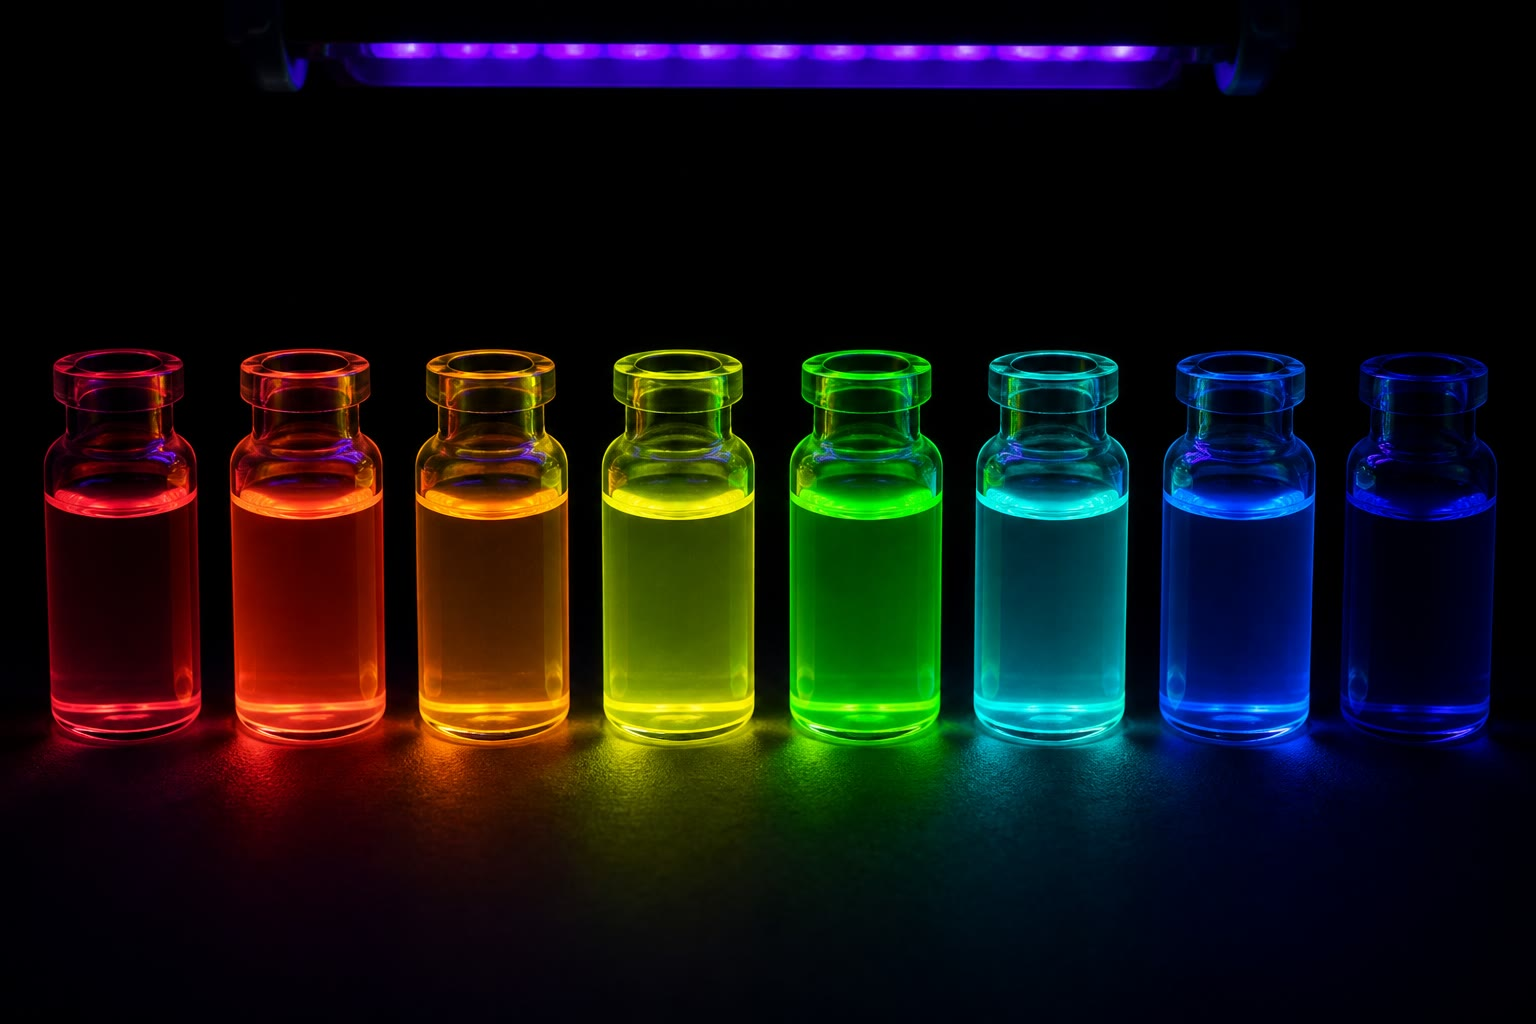
\includegraphics[width=0.58\linewidth]{images/book5/ai/b5-07-quantum-dot-vials.jpg}

{\small 紫外线照射下的量子点：同一种半导体，晶体越来越小，发光颜色由红变蓝。颜色由本章中势箱内粒子的能级决定——限域效应肉眼可见。}
\end{omfigure}

\section{练习}

\begin{exercise}[$\star$]\label{exo:b3:schrodinger-three-dimensions:1}
考虑高斯态 $\psi(\vect r) = A\,\eu^{-r^2/4\sigma^2}$。(a)
归一化（$\int_0^\infty x^2\eu^{-x^2}\dd x = \sqrt\pi/4$）。(b)
计算 $\langle r^2\rangle$ 与 $\Delta x$（可利用各向同性）。(c)
该态的 $\vect\jmath$ 是多少？为什么？(d) 乘以
$\eu^{\iu\vect k_0\cdot\vect r}$：此时 $\langle\vect
p\rangle$ 与 $\vect\jmath$ 各为多少？
\end{exercise}

\begin{exercise}[$\star$]\label{exo:b3:schrodinger-three-dimensions:2}
对于立方势箱，列出 $E = 15$ 以内的所有能级（以
$h^2/8ma^2$ 为单位）及其简并度。然后证明能级 $27$ 的
简并度\emph{超出}了置换所能给出的范围：求出它的两族
量子数，并说明这种“偶然”简并为何不能由
立方对称性导出。
\end{exercise}

\begin{exercise}[$\star$]\label{exo:b3:schrodinger-three-dimensions:3}
计算下列情形的电流 $\vect\jmath$：(a) 平面波
$A\eu^{\iu kx}$；(b) 驻波 $A\sin kx$；(c) 叠加态
$A(\eu^{\iu kx} + r\,\eu^{-\iu kx})$，$r$ 为实数——
将结果解释为入射通量减去反射通量；(d) 环上的态
$A\,\eu^{\iu m\varphi}$，位于半径为 $b$ 的环上（此处取 $|\vect\nabla|
= (1/b)\partial_\varphi$）：一个永远环流的电流。
\end{exercise}

\begin{exercise}[$\star$]\label{exo:b3:schrodinger-three-dimensions:4}
一个量子点微晶将电子–空穴对限制其中，其有效质量为
$\mu = 0.10\,m_{\text{e}}$；其发射光子的能量为体相带隙
$E_{\text{g}} = \qty{1.74}{eV}$ 加上球形势箱的限域能
$\pi^2\hbar^2/2\mu R^2$。(a) 计算
$R = \qty{3}{nm}$ 时的限域能。(b) 求发射光的波长。
(c) 量子点缩小时，颜色向哪个方向变化？
(d) 为什么体相硒化镉（$R$ 较大）只呈现单一的固定颜色？
\end{exercise}

\begin{exercise}[$\star\star$]\label{exo:b3:schrodinger-three-dimensions:5}
一个粒子位于环上（半径为 $b$，坐标为 $\varphi$）：其
定态为 $\psi_m = \eu^{\iu m\varphi}/\sqrt{2\pi}$。(a) 为什么
$m$ 必须为整数？(b) 证明 $E_m = \hbar^2m^2/2mb^2$——
注意两个 $m$ 的区别：写作 $E_m = \hbar^2 m^2/2Mb^2$ 时，
质量为 $M$——并指出每个 $m \neq 0$ 的能级
都是二重简并的：什么对称性使 $+m$ 与 $-m$ 配对？
(c) 计算 $\psi_m$ 的电流，以及粒子带电荷 $q$ 时
相应的“轨道”磁矩。(d) 苯的六个可移动电子位于
半径为 $b \approx \qty{1.4}{\angstrom}$ 的环上：估算第一个允许跃迁
（$m = \pm1 \to \pm2$）的光子能量，并与苯在 \qty{180}{nm}
附近的紫外吸收进行比较——一个环，
不涉及化学。
\end{exercise}

\begin{exercise}[$\star\star$]\label{exo:b3:schrodinger-three-dimensions:6}
各向同性谐振子的简并度。(a) 证明
满足 $n_x + n_y + n_z = n$ 的三元组数为 $(n+1)(n+2)/2$。(b) 列出
$n = 0$ 至 $3$ 的壳层占据数，并计入自旋的二重性。(c) 证明
累积填充数为 $2, 8, 20, 40, \dots$：前三个与
核物理中的“幻数”（额外稳定的核子数）相符——
$40$ 处的失效（真正的幻数是 $28$、$50$）说明
核势的什么性质？(d) 与谐振子不同，盒子的不规则能级
分布为何不产生明显的壳层结构？
\end{exercise}

\begin{exercise}[$\star\star$]\label{exo:b3:schrodinger-three-dimensions:7}
无限深球形势阱（半径 $R$）：利用 $s$ 波技巧，
(a) 求能级 $E_n = n^2\pi^2\hbar^2/2MR^2$ 及波
函数 $u_n$；(b) 计算核子的 $E_1$（$Mc^2 =
\qty{939}{MeV}$），取 $R = \qty{5}{fm}$（使用 $\hbar c =
\qty{197.3}{MeV.fm}$）；(c) 与中等质量核中实测的核子能级
间距（约几 MeV）相比较；(d) 基态中粒子最可能
出现在何处——计算
$|u_1|^2$ 的最大值，并与一维盒子中 $|\varphi|^2$ 的结果对比。
\end{exercise}

\begin{exercise}[$\star\star$]\label{exo:b3:schrodinger-three-dimensions:8}
金属中电子的计数。(a) 由
\cref{prop:b3:schrodinger-three-dimensions:counting}，取两个自旋态，
证明填充 $N$ 个电子于体积 $V$ 中时达到
费米能
\[
E_{\text{F}} = \frac{\hbar^2}{2m_{\text{e}}}\,(3\pi^2n)^{2/3} ,
\qquad n = N/V .
\]
(b) 对铜求值。(c) 计算相应的费米速率
以及费米温度 $E_{\text{F}}/k_{\text{B}}$。(d) 用一句话说明：
为何电子并不全都处于基态，以及
哪一原理（此处预先给出，
在\cref{ch:b3:identical-particles}中证明）禁止了这一点？
\end{exercise}

\begin{exercise}[$\star\star$]\label{exo:b3:schrodinger-three-dimensions:9}
球形势阱的最小深度。对有限深势阱（势能 $-V_0$
，$r < R$ 区域），$s$ 波基态内部为 $u = \sin kr$，外部为
$\eu^{-\kappa r}$。(a) 写出 $k$ 与 $\kappa$ 及匹配条件
$k\cot kR = -\kappa$。(b) 证明束缚态
首次出现于 $kR = \pi/2$ 且恰在 $E = 0$ 时，给出
$V_{0,\min} = \pi^2\hbar^2/8MR^2$。(c) 对氘核求值
（$M \to \mu = m_{\text{p}}/2$，$R = \qty{2.1}{fm}$）。(d)
与一维情形对比，一维中最浅的势阱即可束缚粒子：
$u(0) = 0$ 的壁在物理上改变了什么？
\end{exercise}

\begin{exercise}[$\star\star\star$]\label{exo:b3:schrodinger-three-dimensions:10}
氘核的求解。取 $\mu c^2 = \qty{469}{MeV}$，$R =
\qty{2.1}{fm}$，$B = \qty{2.22}{MeV}$：(a) 计算 $\kappa$（由 $B$
得）及尾长 $1/\kappa$；(b) 写出匹配条件，并证明它化为
$\cot kR = -\kappa/k$，其中 $k$ 由 $V_0 - B$ 确定；
(c) 求 $V_0$（迭代：从 $kR \approx 0.6\pi$ 出发）并
给出 $V_0$（精确到最近的 MeV）；(d) 计算核子间距
大于 $R$ 的概率（对尾部积分），并
评论“一个大部分时间位于自身作用力之外的原子核”。
\end{exercise}

\begin{exercise}[$\star\star\star$]\label{exo:b3:schrodinger-three-dimensions:11}
三维情形下的埃伦费斯特定理与连续性方程。(a) 证明
$\dd\langle\vect r\rangle/\dd t = \langle\vect p\rangle/m$，由
连续性方程出发（对 $\vect r\,\partial_t\rho$ 分部积分）。
(b) 证明 $\dd\langle\vect p\rangle/\dd t =
-\langle\vect\nabla V\rangle$。(c) $V$ 满足什么条件时，
$\langle\vect r\rangle$ 精确地遵循经典轨迹？(d)
给出一个不成立的具体情形（例如被双缝势劈裂的波包），
并说明此时平均值描述的是什么。
%
\end{exercise}

\begin{exercise}[$\star\star\star$]\label{exo:b3:schrodinger-three-dimensions:12}
为什么原子不会坍缩。以试探函数模拟氢原子基态，
取 $\psi \propto \eu^{-r/a}$，其中 $a$ 可调。(a)
承认 $\langle E_k\rangle = \hbar^2/2m_{\text{e}}a^2$ 与
$\langle E_p\rangle = -e^2/4\pi\varepsilon_0a$，解释各项
标度关系的来源。(b) 极小化 $E(a)$，证明最优值为
玻尔半径，此时 $E = \qty{-13.6}{eV}$。(c) 为何将 $a$
缩小到最优值以下会使能量\emph{升高}，尽管势能
变得更深？(d) 把 $1/r$ 换成电子与质子间的引力，
用同样的论证求“引力玻尔半径”，
并由此得出引力为何不能形成
原子。
\end{exercise}

\section{问题：量子点的颜色}

\begin{problem}[{周末问题——通过数纳米尺度
来设计光}]\label{pb:b3:schrodinger-three-dimensions:1}
2023 年诺贝尔化学奖授予了量子点的
发现与合成：晶粒小到使本章“盒中粒子”的
能量决定了它们的颜色，如今在电视屏幕中发光，
并用于标记活细胞中的分子。本题设计一个
基于薛定谔方程的量子点显示器。模型：光学活性的
电子–空穴对，有效质量 $\mu = 0.10\,m_{\text{e}}$
（$m_{\text{e}}c^2 = \qty{511}{keV}$），限制在半径为
$R$ 的球内；发射光子能量为
\[
E(R) = E_{\text{g}} + \frac{\pi^2\hbar^2}{2\mu R^2} ,
\]
其中体相带隙 $E_{\text{g}} = \qty{1.74}{eV}$（硒化镉
）。取 $\hbar c = \qty{197.3}{eV.nm}$，$hc =
\qty{1240}{eV.nm}$。

\medskip\noindent\textbf{第一部分——公式的物理含义。}
\begin{enumerate}
  \item 项 $\pi^2\hbar^2/2\mu R^2$ 从何而来？请推导
        它，即无限深球形势阱的基态能级，利用
        $s$ 波代换。
  \item 为何限域总是使发射能量\emph{升高}，
        而从不降低？
  \item 计算 $R = 10$、$4$、$2$ 与
        \qty{1}{nm}时的限域能，并指出从何种尺寸起它不再是
        $E_{\text{g}}$ 的小修正。
  \item 模型忽略了电子–空穴吸引。若计入该吸引，发射
        能量将沿哪个方向移动，以及为何对\emph{小}量子点忽略它更合理
        （比较 $1/R^2$ 与
        $1/R$ 的标度）？
  \item 体相硒化镉发射的波长是多少？它位于
        光谱的哪一部分？
  \item 为何一杯量子点溶液会以\emph{单一}纯色发光，
        尽管其中含有 $10^{15}$ 个量子点？合成的哪一性质
        得到了验证？
\end{enumerate}

\medskip\noindent\textbf{第二部分——设计调色板。}
显示屏需要红色 \qty{630}{nm}、绿色 \qty{530}{nm}、蓝色
\qty{460}{nm}。
\begin{enumerate}[resume]
  \item 将每个波长换算为光子能量。
  \item 对每种颜色，计算所需的限域能
        以及量子点半径。
  \item 列表给出每个量子点大约有多少个原子宽
        （晶格间距 $\approx \qty{0.6}{nm}$）？
  \item 对硒化镉量子点而言，蓝色最难实现：根据你算出的
        半径，解释原因（当 $R$
        减小时，容差如何变化？）。
  \item 证明发射能量对尺寸的灵敏度为
        \[
        \frac{\dd E}{\dd R} = -\frac{\pi^2\hbar^2}{\mu R^3} ,
        \]
        并以 $\unit{meV}$ 每纳米为单位，在绿色
        量子点的半径处求其数值。
  \item 一批量子点的半径有 $\pm5\%$ 的波动：计算绿光发射的波长
        散布，并与良好显示器所容许的
        $\sim\qty{25}{nm}$ 线宽相比较。
  \item 为什么量子点显示器必须等待能够实现
        \emph{原子尺度}尺寸控制的化学技术——这为何是
        诺贝尔级别的成就？
\end{enumerate}

\medskip\noindent\textbf{第三部分——更亮、更纯、更奇特。}
\begin{enumerate}[resume]
  \item 现代显示屏将量子点用作颜色转换器：蓝色 LED
        照亮红色和绿色量子点。为什么泵浦光子的
        能量必须大于量子点的发射能量？这份差值
        去了哪里？
  \item 计算一个 \qty{460}{nm} 泵浦光子的能量中
        以热的形式损失的比例（当一个 \qty{630}{nm} 红色光子被发射时）。
  \item 量子点可以在多个波长处\emph{吸收}，但
        只能在一个波长处\emph{发射}：请从能级结构出发，解释为什么
        吸收是宽带的，而发射是窄带的。
  \item 生物学家用多种尺寸的量子点标记蛋白质，并用同一盏紫外灯激发它们：
        量子点的何种性质使得一盏灯即可满足需求，
        而有机染料则需要每种颜色一台激光器？
  \item 估算红色量子点中的原子数（$4/3\pi R^3$，
        原子体积 $\sim(\qty{0.3}{nm})^3$）：“人造
        原子”这一名称对于具有分立
        能级、这样大小的物体是否恰当？
  \item 用一句话回答：在这个人造原子中，什么扮演了“原子核”的角色
        ——即是什么束缚着电子？
\end{enumerate}

\medskip\noindent\textbf{第四部分——贯穿物理学的限域。}
\begin{enumerate}[resume]
  \item 将同一估算式 $E_1 \sim \pi^2\hbar^2/2MR^2$ 应用于
        $R = \qty{3}{fm}$ 的核子，得到的能量量级是多少？（这正是
        核物理使用 MeV 作单位的原因。）
  \item 将其应用于限制在原子核尺度内的电子，得到
        多么惊人的能量？这说明原子核“内部”
        的电子有何问题（这一论证曾经
        推翻了一种 β 衰变理论）？
  \item 将其应用于你自己（\qty{70}{kg}）处于 \qty{2}{m} 的房间中：计算
        限域能，并作出结论。
  \item 反推该公式：限域尺寸为多大时，
        \emph{电子}的限域能达到其静能
        $m_{\text{e}}c^2$？这时出现的何种新物理
        （粒子对的产生，见\cref{ch:b3:relativistic-dynamics}）表明
        单粒子薛定谔方程此时
        已超出其适用范围？
  \item 给出一般的标度律：限域能与
        质量、与尺寸的关系。
  \item 概括这一命名结果：一个公式
        $E_{\text{g}} + \pi^2\hbar^2/2\mu R^2$，将半径
        $4.0$、$2.5$ 和 \qty{2.0}{nm} 分别转化为红、绿、蓝——
        通过数纳米设计颜色，在任何
        电子产品商店都能买到。
\end{enumerate}
\end{problem}
